\section{Программы}
\subsection{Программа 1}
\begin{lstlisting}[caption={Исходный код Программы 1}]
#include <fcntl.h>
#include <stdio.h>

int main() {
		FILE *fs1, *fs2;
		char buff1[20], buff2[20], c;
		int flag1 = 1, flag2 = 1;
		int fd = open("alphabet.txt", O_RDONLY);
		fs1 = fdopen(fd, "r");
		setvbuf(fs1, buff1, _IOFBF, 20);
		fs2 = fdopen(fd, "r");
		setvbuf(fs2, buff2, _IOFBF, 20);
		while (flag1 == 1 || flag2 == 1) {
				flag1 = fscanf(fs1, "%c", &c);
				if (flag1 == 1)
				fprintf(stdout, "%c", c);
				flag2 = fscanf(fs2, "%c", &c);
				if (flag2 == 1)
				fprintf(stdout, "%c", c);
			}
		fprintf(stdout, "\n");
		return 0;
	}
\end{lstlisting}

Скриншот результата выполнения программы 1 представлен на рисунке \ref{img:1.png}.
\jimg{1.png}{Результат выполнения программы 1}

\clearpage

\textbf{Анализ полученного результата}

При запуске программы системный вызов open() открывает файл alphabet.txt в режиме O\_RDONLY, в результате чего в пространстве ядра формируется структура struct file. Ссылка на неё заносится в таблицу файловых дескрипторов текущего процесса под индексом 3, поскольку младшие дескрипторы 0, 1 и 2 по умолчанию закреплены за стандартными потоками stdin, stdout и stderr. Этот индекс возвращается в качестве значения переменной fd.

Далее библиотечная функция fdopen() связывает дескриптор fd с двумя логическими потоками fs1 и fs2, создавая для каждого структуру FILE (фактически struct \_IO\_FILE), в которой поле \_fileno принимает значение fd. С помощью функции setvbuf() для обоих потоков fs1 и fs2 устанавливается режим полной буферизации (\_IOFBF) со своим пользовательским буфером размером 20 байт (buff1 и buff2 соответственно).

Первый вызов fscanf() для fs1 приводит к заполнению буфера buff1 первыми 20 байтами файла (символами от a до t). В системной структуре file при этом сдвигается указатель текущей позиции f\_pos на 20. Из буфера buff1 извлекается символ a, сохраняется в c и выводится на экран, а локальный указатель чтения \_IO\_read\_ptr для fs1 перемещается на один байт вперед.

Поскольку потоки fs1 и fs2 используют общий файловый дескриптор, они разделяют одну структуру file и текущую позицию f\_pos. Поэтому при первом вызове fscanf() для fs2 чтение в буфер buff2 начинается с позиции f\_pos = 20. В буфер buff2 считываются оставшиеся 6 символов файла (от u до z), а f\_pos увеличивается до конца файла. Символ u извлекается из buff2 и записывается в стандартный вывод.

В последующих шагах цикла символы попеременно считываются из уже заполненных буферов buff1 и buff2. После того как буфер buff2 будет полностью исчерпан (когда \_IO\_read\_ptr сравняется с \_IO\_read\_end), программа продолжит считывать и выводить оставшиеся символы исключительно из буфера buff1 (вплоть до t), пока и в нём не закончатся данные.

На рисунке \ref{img:1.pdf} отображены связи структур для программы 1.

\begin{figure}[H]
	\center{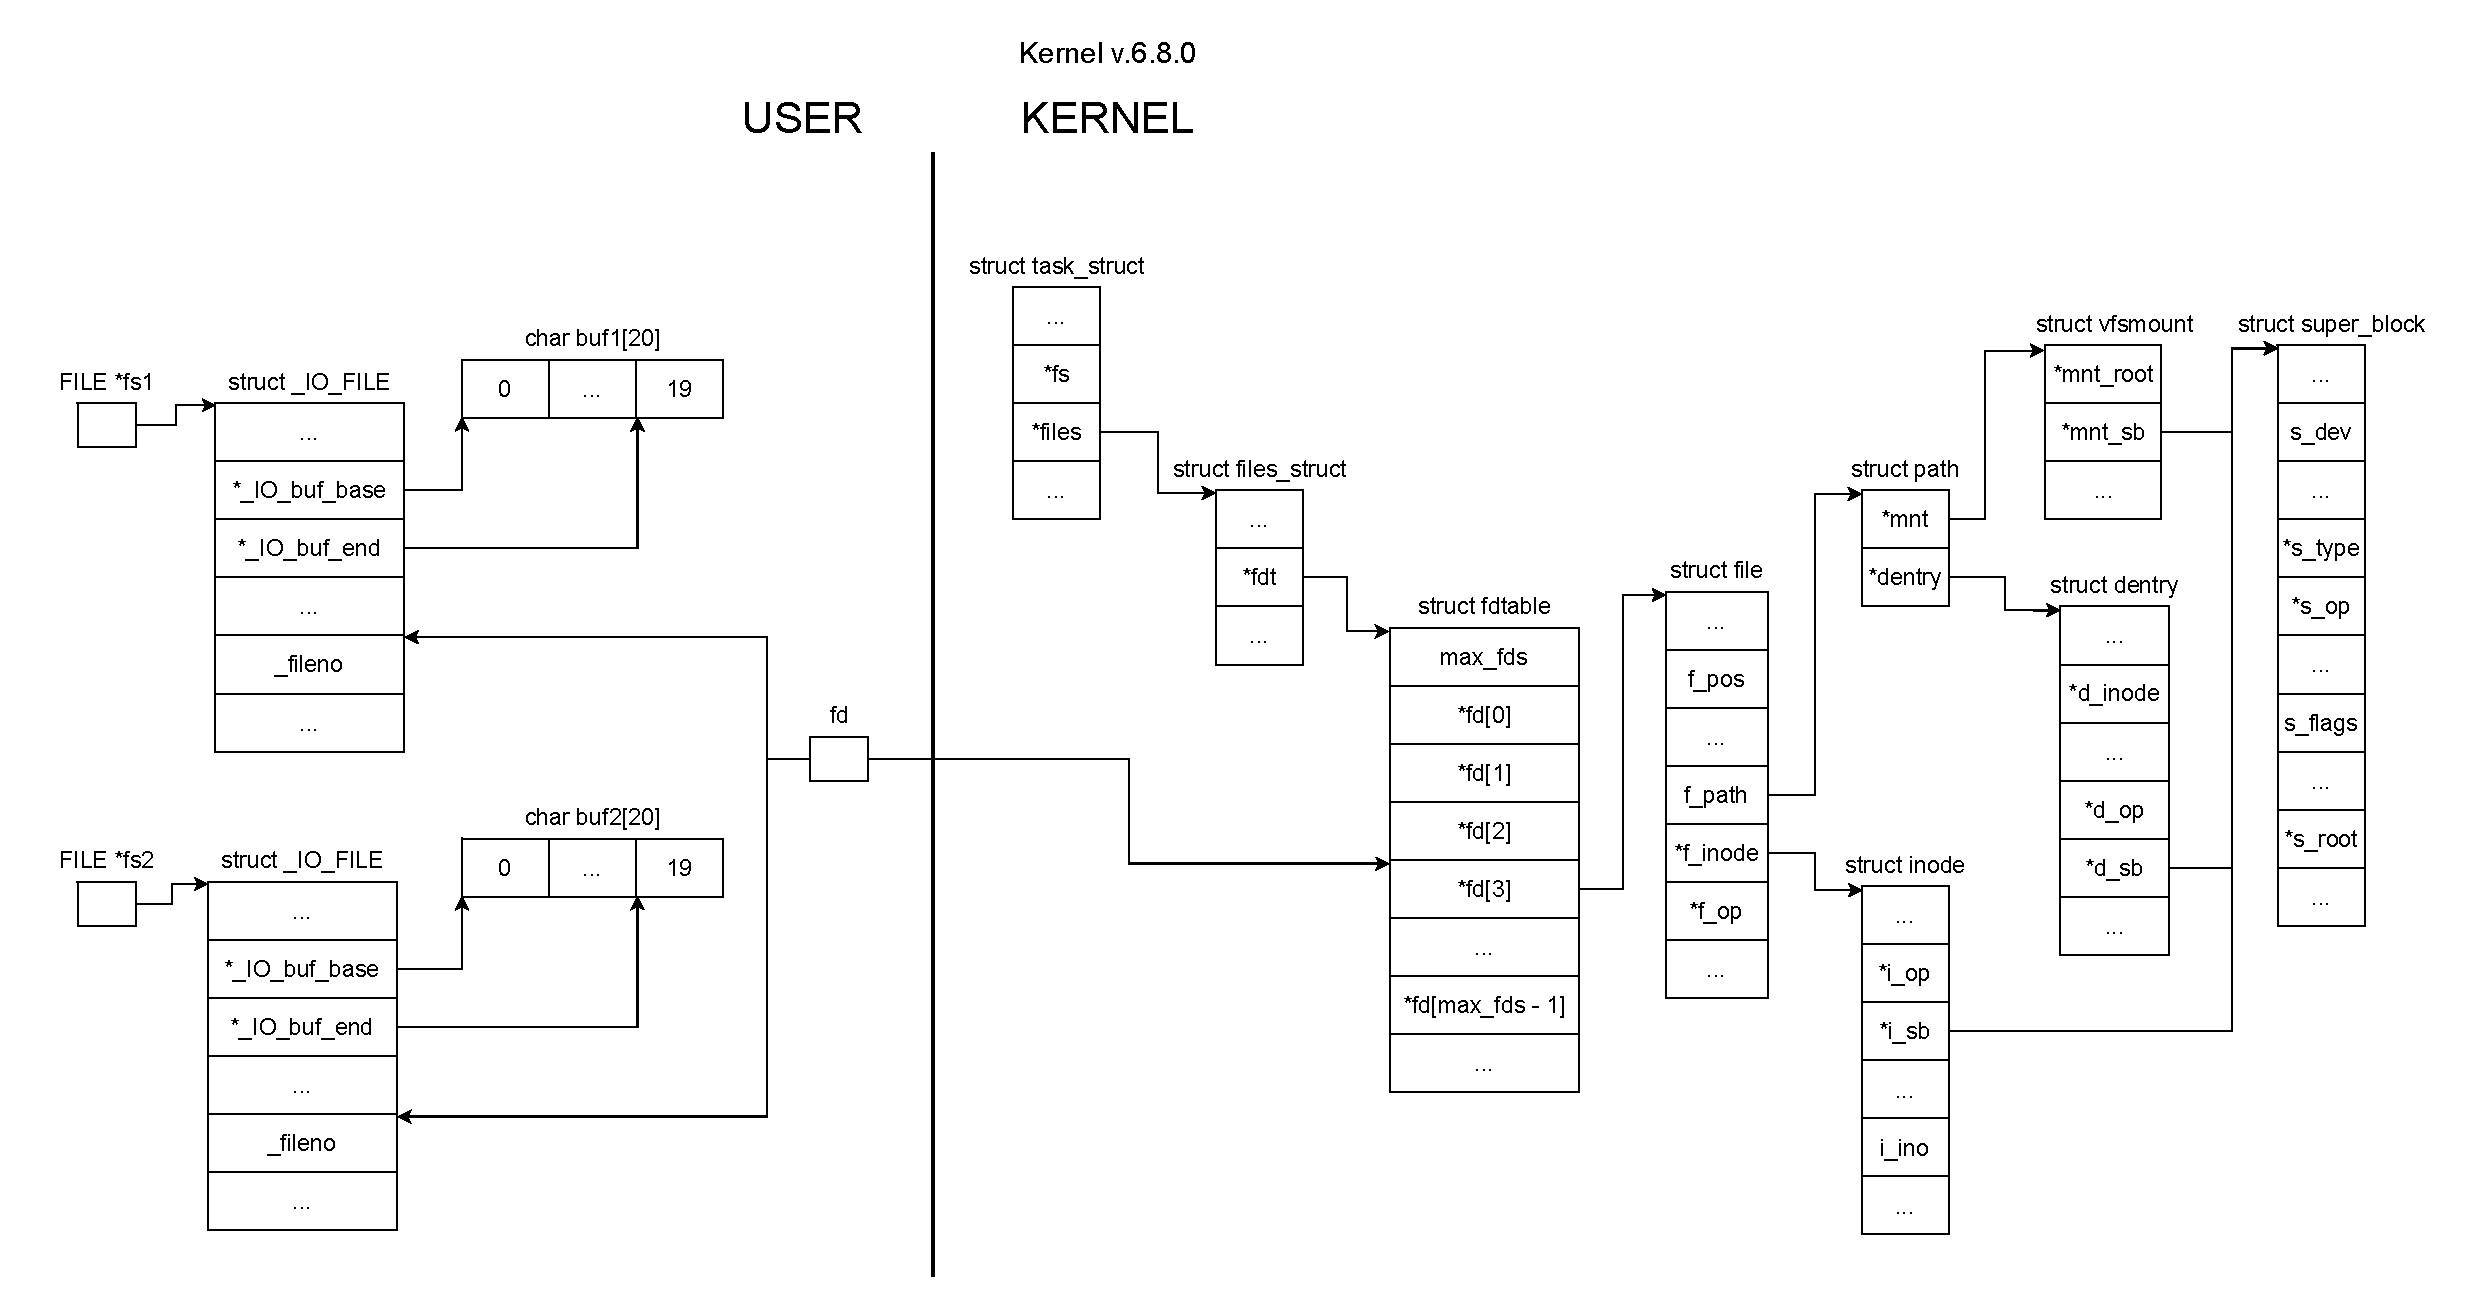
\includegraphics[width=\textwidth, trim=0cm 0cm 0cm 1.3cm, clip]{img/1.pdf}}
	\caption{Схема связи структур для программы 1}
	\label{img:1.pdf}
\end{figure}

\subsection{Программа 2}
\subsubsection{Один поток}
\begin{lstlisting}[caption={Исходный код однопоточной Программы 2}]
#include <fcntl.h>
#include <unistd.h>

int main() {
    char c;
    int flag1 = 1, flag2 = 1;
    int fd1 = open("alphabet.txt", O_RDONLY);
    int fd2 = open("alphabet.txt", O_RDONLY);
    while (flag1 == 1 && flag2 == 1) {
        flag1 = read(fd1, &c, 1);
        if (flag1 == 1) {
            write(1, &c, 1);
            flag2 = read(fd2, &c, 1);
            if (flag2 == 1)
                write(1, &c, 1);
        }
    }
    close(fd1);
    close(fd2);
    c = '\n';
    write(1, &c, 1);
    return 0;
}
\end{lstlisting}

Скриншот результата выполнения однопоточной программы 2 представлен на рисунке \ref{img:2.png}.
\jimg{2.png}{Результат выполнения однопоточной программы 2}

\textbf{Анализ полученного результата}


С помощью двух системных вызовов open() программа открывает файл alphabet.txt в режиме O\_RDONLY, возвращая дескрипторы fd1 и fd2. В таблице файлов процесса под номерами 3 и 4 (поскольку дескрипторы 0, 1 и 2 заняты стандартными потоками ввода-вывода) создаются записи, указывающие на две независимые системные структуры struct file в ядре. Обе эти структуры указывают на общий inode одного и того же файла.

Каждая структура struct file обладает собственным указателем текущего смещения f\_pos, который изначально равен нулю. Системный вызов read() для fd1 считывает из файла один символ (символ a), сдвигая f\_pos в первой структуре file на 1, после чего символ отправляется в стандартный вывод через write().

Второй вызов read() использует дескриптор fd2, у которого f\_pos во второй структуре file по-прежнему равен 0. Из-за этого из файла считывается тот же самый символ a, и f\_pos во второй структуре увеличивается на 1.

Процесс поочередного чтения через fd1 и fd2 продолжается в цикле до тех пор, пока f\_pos в обеих структурах не достигнет конца файла (размера в 26 байт). Благодаря независимости файловых позиций, каждый символ последовательно читается и выводится по два раза, что дает строго детерминированный результат: aabbcc...zz.

\clearpage

\subsubsection{Один основной поток и один дополнительный поток}
\begin{lstlisting}[caption={Исходный код Программы 2 с одним дополнительным потоком}]
#include <fcntl.h>
#include <unistd.h>
#include <pthread.h>

int flag1 = 1, flag2 = 1;

void* thread1_func(void* arg) {
    char c;
    int fd = *(int*)arg;
    while (flag1 == 1 && flag2 == 1) {
        flag1 = read(fd, &c, 1);
        if (flag1 == 1) {
            write(1, &c, 1);
        }
    }
    close(fd);
    return NULL;
}

int main() {
    char c;
    pthread_t t1, t2;
    int fd1 = open("alphabet.txt", O_RDONLY);
    int fd2 = open("alphabet.txt", O_RDONLY);
    pthread_create(&t1, NULL, thread1_func, &fd1);
    while (flag1 == 1 && flag2 == 1) {
        flag2 = read(fd2, &c, 1);
        if (flag2 == 1) {
            write(1, &c, 1);
        }
    }
    close(fd2);
    pthread_join(t1, NULL);
    c = '\n';
    write(1, &c, 1);
    return 0;
}
\end{lstlisting}

Скриншот результата выполнения программы 2 с одним дополнительным потоком представлен на рисунке \ref{img:2_1thread.png}.
\jimg{2_1thread.png}{Результат выполнения программы 2 с одним дополнительным потоком}

\textbf{Анализ полученного результата}

В данном варианте главный поток с помощью pthread\_create() порождает дополнительный поток исполнения, передавая ему указатель на дескриптор fd1. Процедура создания нового потока операционной системой занимает некоторое время. В этот промежуток главный поток, выполняющий чтение через fd2, может успеть прочесть и вывести на экран как часть файла, так и весь его объем целиком.

После того как порожденный поток переходит в активное состояние, чтение данных через независимые файловые дескрипторы и их вывод производятся обоими потоками параллельно. Очередность выполнения их операций ввода-вывода полностью определяется планировщиком операционной системы.

Каждый символ из файла будет гарантированно прочитан и выведен дважды (по одному разу каждым из потоков), но их взаимное расположение в выходной строке недетерминировано и зависит от особенностей распределения квантов процессорного времени между потоками.

\clearpage

\subsubsection{Два дополнительных потока}
\begin{lstlisting}[caption={Исходный код Программы 2 с двумя дополнительными потоками}]
#include <fcntl.h>
#include <unistd.h>
#include <pthread.h>

int flag1 = 1, flag2 = 1;

void* thread1_func(void* arg) {
    char c;
    int fd = *(int*)arg;
    while (flag1 == 1 && flag2 == 1) {
        flag1 = read(fd, &c, 1);
        if (flag1 == 1) {
            write(1, &c, 1);
        }
    }
    close(fd);
    return NULL;
}

void* thread2_func(void* arg) {
    char c;
    int fd = *(int*)arg;
    while (flag1 == 1 && flag2 == 1) {
        flag2 = read(fd, &c, 1);
        if (flag2 == 1) {
            write(1, &c, 1);
        }
    }
    close(fd);
    return NULL;
}

int main() {
    char c = '\n';
    pthread_t t1, t2;
    int fd1 = open("alphabet.txt", O_RDONLY);
    int fd2 = open("alphabet.txt", O_RDONLY);
    pthread_create(&t1, NULL, thread1_func, &fd1);
    pthread_create(&t2, NULL, thread2_func, &fd2);
    pthread_join(t1, NULL);
    pthread_join(t2, NULL);
    write(1, &c, 1);
    return 0;
}
\end{lstlisting}

Скриншот результата выполнения программы 2 с двумя дополнительными потоками представлен на рисунке \ref{img:2_2thread.png}.
\jimg{2_2thread.png}{Результат выполнения программы 2 с двумя дополнительными потоками}

\textbf{Анализ полученного результата}

Главный поток создает два дочерних потока с помощью последовательных вызовов pthread\_create(), передавая первому указатель на fd1, а второму — на fd2. Сам главный поток после этого блокируется на вызовах pthread\_join(), дожидаясь их завершения.

Инициализация и запуск потоков требуют системного времени, и порядок, в котором они приступят к выполнению своих функций, заранее не предопределен. Логика планировщика задач операционной системы полностью управляет распределением ресурсов между этими потоками.

В результате оба потока параллельно читают весь файл с самого начала (поскольку структуры struct file в ядре у них независимы и имеют собственные смещения f\_pos), выводя символы в общий стандартный поток. Итоговая строка содержит по два каждого символа, но их последовательность носит случайный характер.


На рисунке \ref{img:2.pdf} отображены связи структур для программы 2.

\begin{figure}[H]
	\center{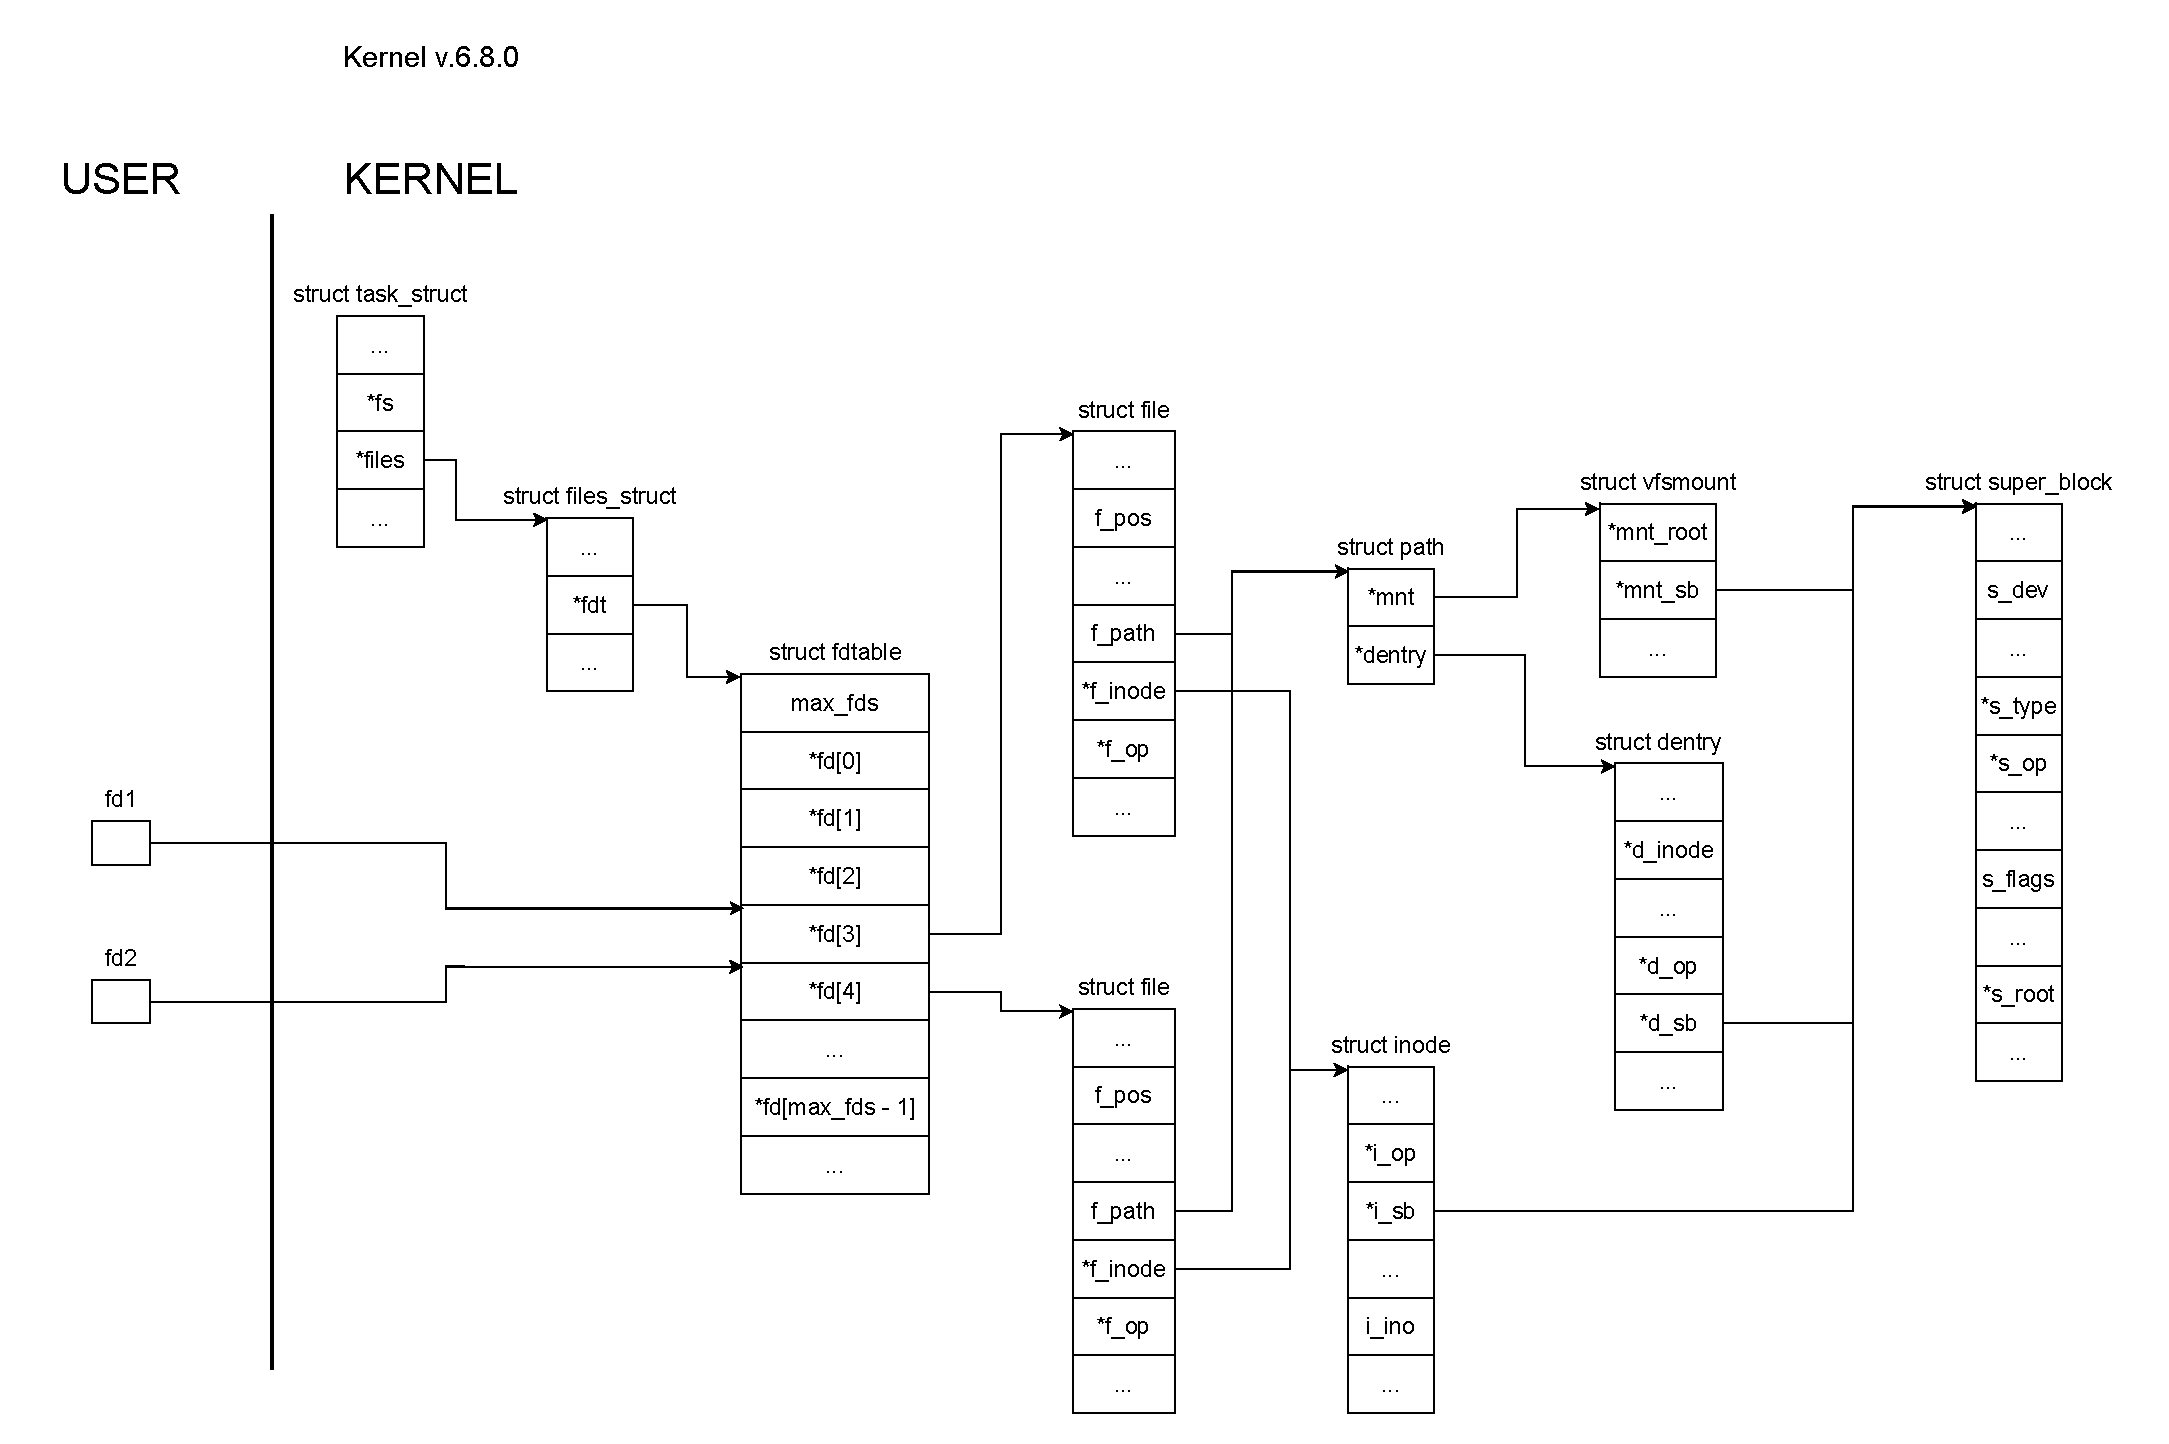
\includegraphics[width=\textwidth, trim=0cm 0cm 0cm 1.3cm, clip]{img/2.pdf}}
	\caption{Схема связи структур для программы 2}
	\label{img:2.pdf}
\end{figure}


\subsection{Программа 3}
\subsubsection{Небуферизованный ввод-вывод}
\begin{lstlisting}[caption={Исходный код Программы 3 с небуферизованным вводом-выводом}]
#include <fcntl.h>
#include <unistd.h>
#include <sys/stat.h>
#include <stdio.h>

void print_stat(char *msg) {
    struct stat statbuf;
    stat("q.txt", &statbuf);
    fprintf(stdout, "%s: inode = %ld, size = %ld bytes\n", msg, statbuf.st_ino, statbuf.st_size);
}

int main() {
    int fd1 = open("q.txt", O_RDWR);
    print_stat("open fd1");
    int fd2 = open("q.txt", O_RDWR);
    print_stat("open fd2");
    for (char c = 'a'; c <= 'z'; c++) {
        if (c % 2)
            write(fd1, &c, 1);
        else
            write(fd2, &c, 1);
        print_stat("write");
    }
    close(fd1);
    print_stat("close fd1");
    close(fd2);
    print_stat("close fd2");
    return 0;
}
\end{lstlisting}

Скриншот результата выполнения программы 3 с небуферизованным вводом-выводом представлен на рисунке \ref{img:3_write.png}.
\img{12cm}{3_write.png}{Результат выполнения программы 3 с небуферизованным вводом-выводом}

\clearpage

\textbf{Анализ полученного результата}

При выполнении двух системных вызовов open() с флагом O\_RDWR (в режииме <<чтения - записи>>) создаются два файловых дескриптора (fd1 и fd2) с номерами 3 и 4. Соответствующие им независимые структуры struct file в ядре указывают на один inode файла q.txt, но при этом обладают разными значениями текущей позиции f\_pos, изначально равными нулю.

На первом шаге цикла вызов write() для fd1 записывает символ a в начало файла, сдвигая f\_pos в первой структуре file на 1. Текущий размер q.txt становится равным 1 байту.

На втором шаге цикла выполняется запись через дескриптор fd2. Поскольку f\_pos во второй структуре file все еще равен 0, системный вызов write() перезаписывает ранее сохраненный символ a символом b. Размер файла при этом не увеличивается и остается равным 1 байту, а f\_pos для fd2 сдвигается на 1.

Подобное поочередное перекрытие символов продолжается на протяжении всей работы цикла. Символы, записываемые через fd1, заменяются символами, отправляемыми через fd2.

В результате в q.txt сохраняются только четные буквы алфавита (b, d, f...), начиная с b, а финальный размер файла составляет 13 байт (половина алфавита).


\subsubsection{Буферизованный ввод-вывод}
\begin{lstlisting}[caption={Исходный код Программы 3 с буферизованным вводом-выводом}]
#include <fcntl.h>
#include <stdio.h>
#include <sys/stat.h>

void print_stat(char *msg) {
    struct stat statbuf;
    stat("q.txt", &statbuf);
    fprintf(stdout, "%s: inode = %ld, size = %ld bytes\n", msg, statbuf.st_ino, statbuf.st_size);
}

int main() {
    FILE *fs1 = fopen("q.txt", "w");
    print_stat("fopen fs1");
    FILE *fs2 = fopen("q.txt", "w");
    print_stat("fopen fs2");
    for (char c = 'a'; c <= 'z'; c++) {
        if (c % 2)
            fprintf(fs1, "%c", c);
        else
            fprintf(fs2, "%c", c);
        print_stat("fprintf");
    }
    fclose(fs1);
    print_stat("fclose fs1");
    fclose(fs2);
    print_stat("fclose fs2");
    return 0;
}
\end{lstlisting}

Скриншот результата выполнения программы 3 с буферизованным вводом-выводом представлен на рисунке \ref{img:3_fprintf.png}.
\img{12cm}{3_fprintf.png}{Результат выполнения программы 3 с буферизованным вводом-выводом}

\clearpage

\textbf{Анализ полученного результата}

Функция fopen() в режиме "w"\ открывает файл q.txt дважды, возвращая указатели на две структуры FILE (fs1 и fs2), ассоциированные с независимыми дескрипторами 3 и 4. В пространстве ядра для них создаются две структуры struct file, указывающие на один inode. При этом библиотека stdio.h выделяет в пользовательском пространстве для каждого потока собственный буфер размером 4096 байт.

При выполнении цикла вызовы fprintf() записывают данные исключительно в эти локальные буферы, не выполняя немедленных системных вызовов записи в ядро. В буфере fs1 накапливаются нечетные символы алфавита (начиная с a), а в буфере fs2 — четные (начиная с b). Соответствующие указатели \_IO\_WRITE\_PTR смещаются в памяти на 13 байт.

Запись данных на диск происходит при вызове fclose(). Сначала закрывается поток fs1. Накопленные 13 байт из буфера fs1 записываются в файл q.txt с нулевой позиции (так как f\_pos дескриптора 3 равен 0). Размер файла становится равен 13 байтам, а f\_pos для первого дескриптора увеличивается до 13.

Затем вызывается fclose() для fs2. Поскольку позиция f\_pos во второй структуре file (соответствующей дескриптору 4) все еще равна 0, 13 байт из буфера fs2 записываются также с начала файла. Это перезаписывает данные, ранее сохраненные из fs1. Итоговый размер файла q.txt остается равным 13 байтам, но его содержимое теперь состоит только из символов буфера fs2 (bdfhjlnprtvxz). Таким образом, результат зависит от порядка вызова функций закрытия потоков.


На рисунке \ref{img:3.pdf} отображены связи структур для программы 3 с буферизованным вводом-выводом.

\begin{figure}[H]
	\center{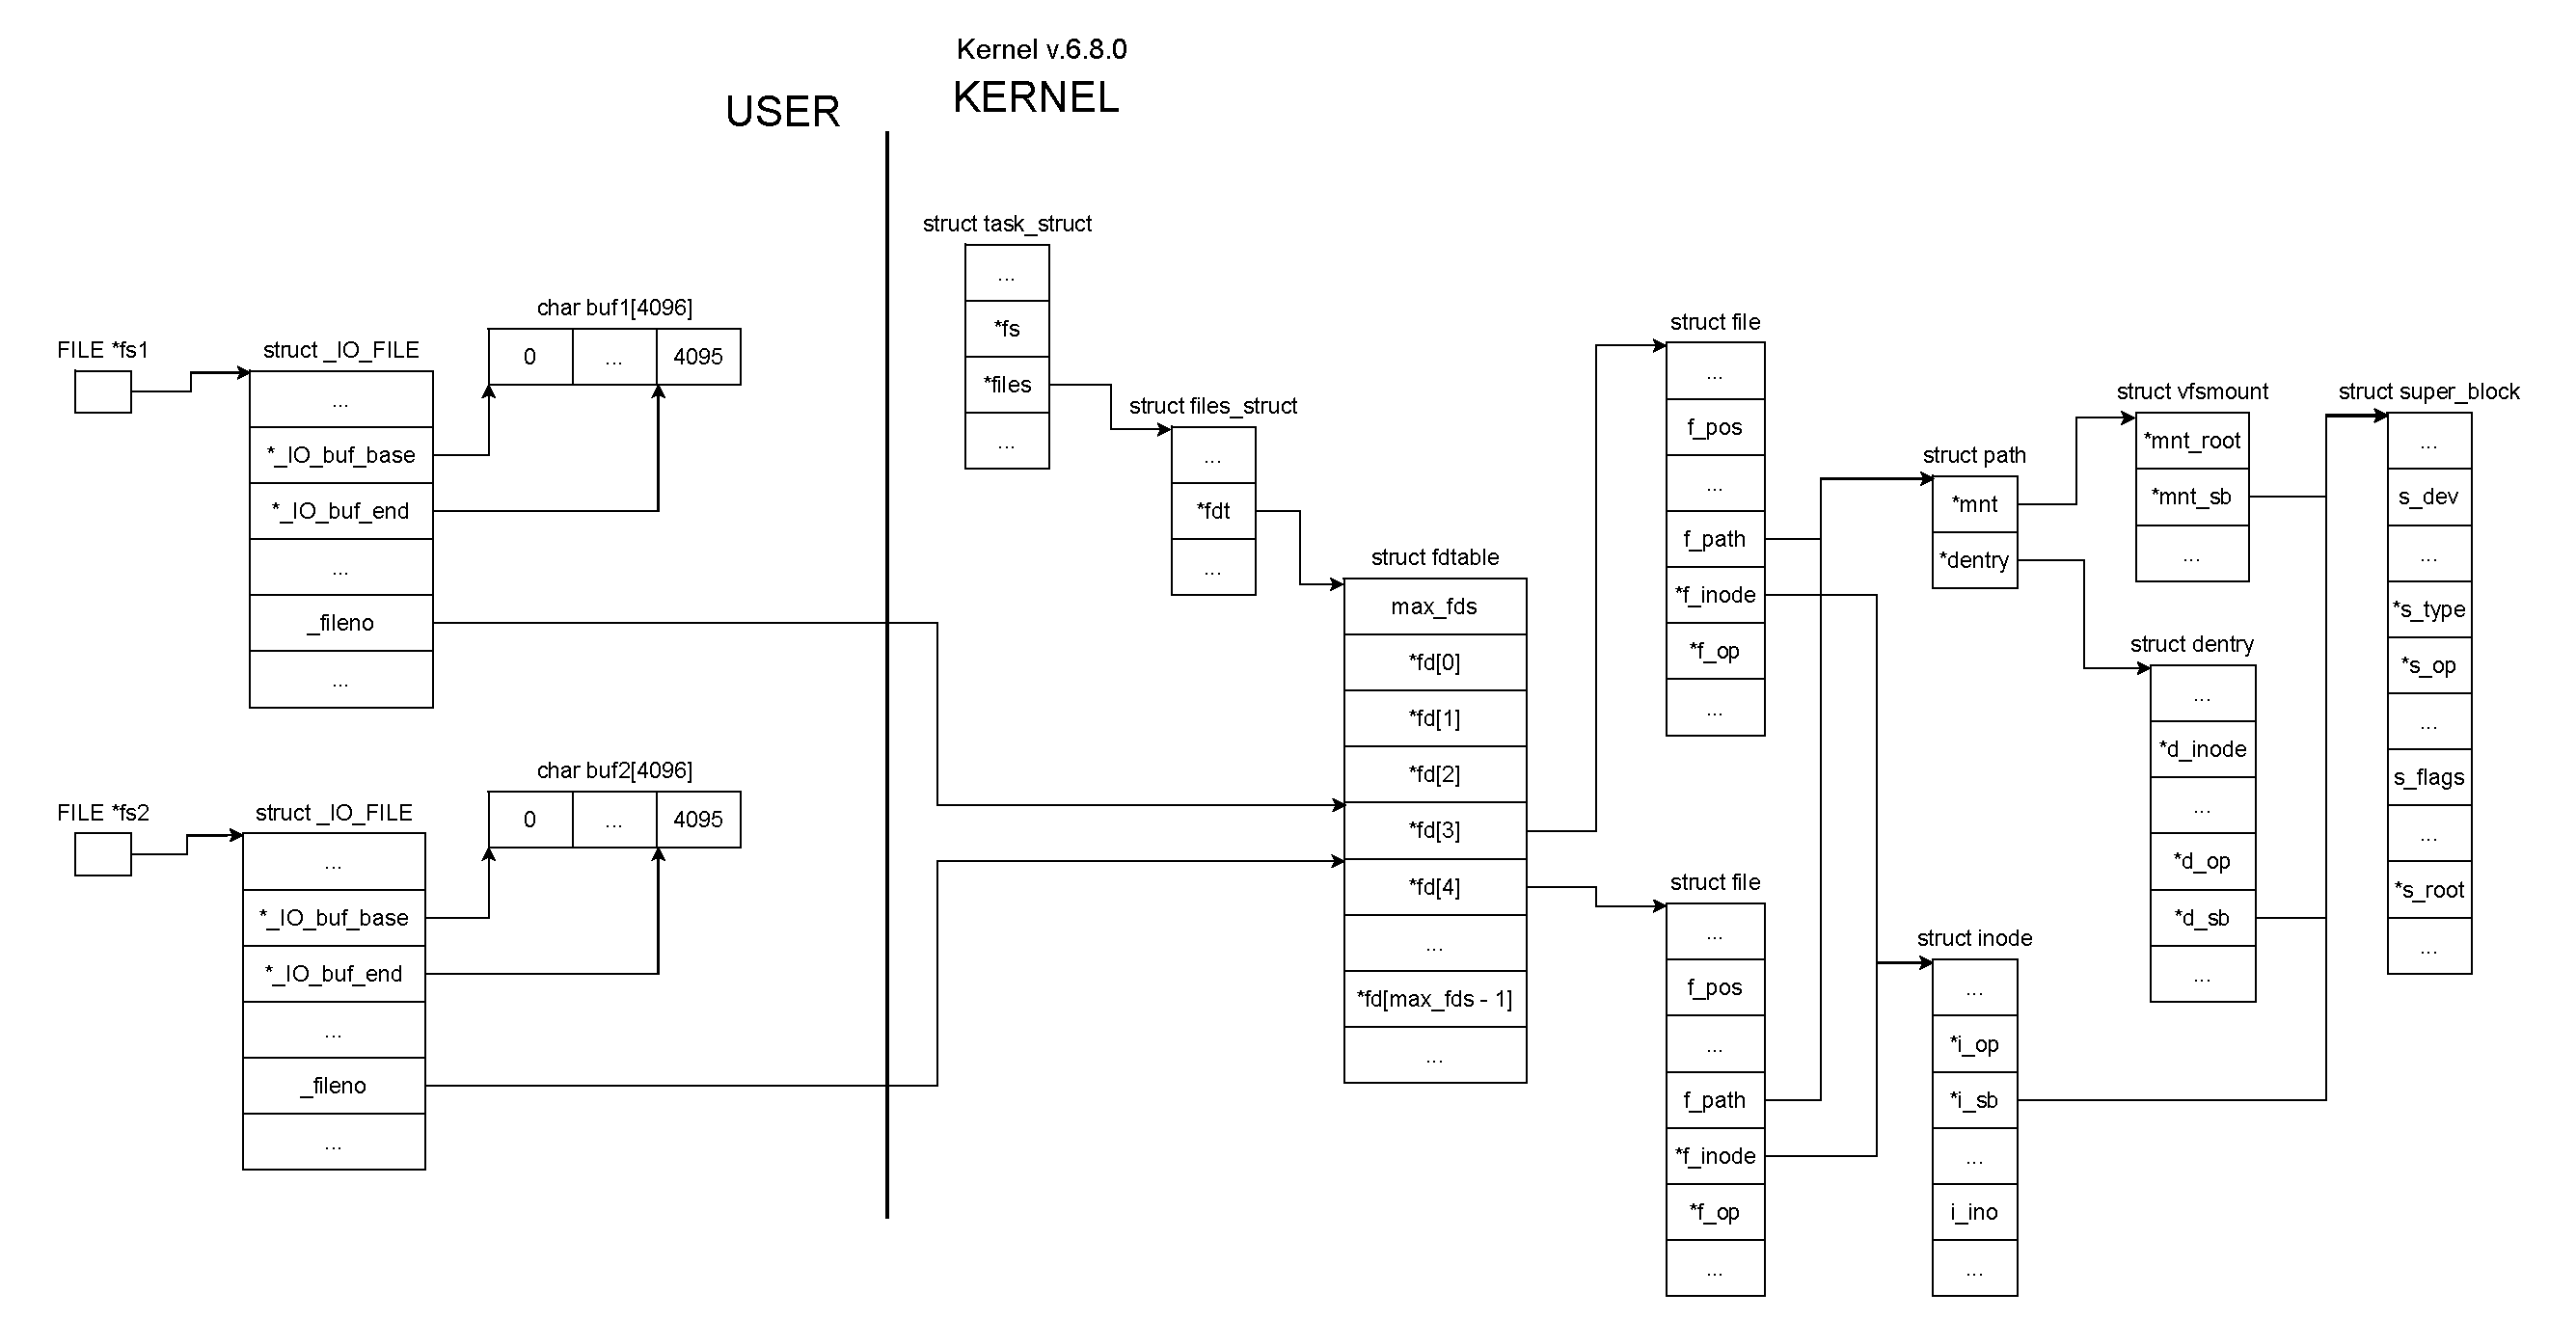
\includegraphics[width=\textwidth, trim=0cm 0cm 0cm 1.3cm, clip]{img/3.pdf}}
	\caption{Схема связи структур для программы 3 с буферизованным вводом-выводом}
	\label{img:3.pdf}
\end{figure}

\subsubsection{Вывод}
Для предотвращения потери и взаимной перезаписи данных при работе с одним файлом через несколько независимых дескрипторов необходимо использовать режим дозаписи (append):

1. В небуферизованном вводе-выводе (системный вызов open) следует использовать флаг \texttt{O\_APPEND} (в сочетании с \texttt{O\_WRONLY} или \texttt{O\_RDWR}). Данный флаг гарантирует смещение указателя текущей позиции ядра (\texttt{f\_pos}) в конец файла перед каждым вызовом \texttt{write()}, что исключает перезапись ранее записанных данных другими дескрипторами.

2. В буферизованном вводе-выводе (функция fopen) файл необходимо открывать в режиме \texttt{"a"} или \texttt{"a+"}. Этот режим на уровне ядра добавляет флаг \texttt{O\_APPEND}. При вызове функций очистки и закрытия потоков (\texttt{fflush} или \texttt{fclose}) данные из пользовательских буферов будут гарантированно дописаны в конец файла, а не записаны поверх нового содержимого.
